% ======================================================================
%  Chapter 13 — Floquet Light  (EXPANDED)
% ======================================================================

\section{Time as a new degree of freedom}
\label{sec:ch13-time}

All the topological photonic systems discussed so far have been
\emph{static}: the material matrix $\Mmat(\rvec)$ is time-independent,
and topology arises from the spatial periodicity of the photonic
crystal.  A fundamentally different approach uses \emph{temporal
modulation}: periodically varying the material parameters in time to
create an effective gauge field for photons.

The mathematical framework for time-periodic systems is \emph{Floquet
theory}, the temporal analog of Bloch theory for spatially periodic
systems \cite{ozawa2018topological}.  Just as spatial periodicity defines Bloch bands labelled by
a crystal momentum $\kvec$, temporal periodicity defines Floquet
quasi-energy bands labelled by a quasi-energy $\varepsilon$
\cite{zhong2024topological}.  These
Floquet bands can carry their own topological invariants, leading to
``Floquet topological insulators'' for light
\cite{zhang2021proposal}.

The Floquet approach is especially appealing because it can break the
effective time-reversal symmetry of the Floquet eigenproblem
\emph{without} magneto-optical materials.  The symmetry breaking comes
from the modulation phases, which can be engineered with standard
electro-optic or acoustic components.

\section{Floquet theory for Maxwell equations}
\label{sec:ch13-floquet-theory}

\subsection{Time-periodic material parameters}
\label{sec:ch13-time-periodic}

Consider a photonic system whose material matrix is periodically
modulated in time:
\begin{equation}\label{eq:ch13-time-periodic}
  \Mmat(\rvec,t) = \Mmat(\rvec,t+T)\,,
\end{equation}
where $T=2\pi/\Omega_{\mathrm{mod}}$ is the modulation period and
$\Omega_{\mathrm{mod}}$ is the modulation frequency.  In practice, the
modulation might be achieved through electro-optic modulation of the
refractive index, acoustic waves creating a travelling refractive-index
grating, parametric coupling between resonator modes, or mechanical
modulation of a metamaterial geometry.

\subsection{Floquet's theorem}
\label{sec:ch13-floquet-theorem}

Floquet's theorem is the temporal analog of Bloch's theorem.  It states
that the solutions of a linear differential equation with
$T$-periodic coefficients can be written in the form
\begin{equation}\label{eq:ch13-floquet-form}
  \emfield(\rvec,t) = \ee^{-\ii\varepsilon t}\,
  \mathbf{v}(\rvec,t)\,,
  \qquad \mathbf{v}(\rvec,t+T) = \mathbf{v}(\rvec,t)\,,
\end{equation}
where $\varepsilon$ is the \emph{quasi-energy} and $\mathbf{v}$ is
time-periodic.  The quasi-energy plays the role of energy in
time-independent systems, but with the crucial difference that it is
defined only modulo $\Omega_{\mathrm{mod}}$: the quasi-energies
$\varepsilon$ and $\varepsilon+n\Omega_{\mathrm{mod}}$ ($n\in\mathbb{Z}$)
describe the same physical state.  This periodicity is the temporal
analog of the crystal momentum being defined modulo a reciprocal
lattice vector.

\subsection{The Floquet--Bloch eigenproblem}
\label{sec:ch13-floquet-bloch}

Expanding the time-periodic function $\mathbf{v}$ in Fourier harmonics
\cite{ozawa2018topological},
\begin{equation}\label{eq:ch13-fourier-expansion}
  \mathbf{v}(\rvec,t) = \sum_{m=-\infty}^{\infty}
  \mathbf{v}_m(\rvec)\,\ee^{-\ii m\Omega_{\mathrm{mod}}t}\,,
\end{equation}
and substituting into the Maxwell equations gives a coupled system of
static equations for the Fourier components:
\begin{equation}\label{eq:ch13-floquet-static}
  \sum_{m'}\bigl[
    \Maxop\,\delta_{mm'} - (\varepsilon+m\Omega_{\mathrm{mod}})\,
    \Mmat_{m-m'}(\rvec)
  \bigr]\mathbf{v}_{m'}(\rvec) = 0\,,
\end{equation}
where $\Mmat_m(\rvec)=T^{-1}\int_0^T\Mmat(\rvec,t)
\ee^{\ii m\Omega_{\mathrm{mod}}t}\,\dd t$ are the Fourier components of
the material matrix.

This is an infinite-dimensional eigenproblem in the combined
space-and-harmonic indices, analogous to the plane-wave expansion in
the spatial case.  In practice, the Fourier series is truncated to
$|m|\leq M_{\max}$, giving a finite matrix of dimension
$(2M_{\max}+1)$ times the spatial degrees of freedom.  The eigenvalues
are the Floquet quasi-energies.

\subsection{The Floquet Brillouin zone}
\label{sec:ch13-floquet-bz}

Because the quasi-energy is periodic with period $\Omega_{\mathrm{mod}}$,
it lives in a ``Floquet Brillouin zone''
$\varepsilon\in[-\Omega_{\mathrm{mod}}/2,\Omega_{\mathrm{mod}}/2)$.
If the system also has spatial periodicity, the quasi-energies depend on
the Bloch wavevector $\kvec$, and the full band structure is defined on
the product of the spatial Brillouin zone and the Floquet Brillouin zone.

This periodicity has a profound consequence: there are \emph{two}
distinct types of gaps in the Floquet spectrum.  The gap at
$\varepsilon=0$ (centre of the Floquet zone) is analogous to a gap in
a static band structure.  But there is also a gap at
$\varepsilon=\pm\Omega_{\mathrm{mod}}/2$ (edge of the Floquet zone),
which has no static analog.  Both gaps can host topological edge modes.

\section{Effective gauge fields from modulation}
\label{sec:ch13-gauge-fields}

\subsection{The coupled-resonator picture}
\label{sec:ch13-coupled-resonator}

The key insight of Floquet topological photonics is that a suitably
designed temporal modulation can create an \emph{effective gauge field}
for photons.  The mechanism is most transparent in a lattice of coupled
resonators.

Consider a 2D lattice of optical resonators with resonance frequency
$\omega_0$.  In the absence of modulation, the coupling between
resonators $i$ and $j$ is described by a real hopping amplitude
$J_0$, and the tight-binding Hamiltonian is time-reversal invariant.

Now suppose the coupling is modulated with a spatially varying phase:
\begin{equation}\label{eq:ch13-modulated-coupling}
  J_{ij}(t) = J_0\cos\bigl(\Omega_{\mathrm{mod}}t + \phi_{ij}\bigr)\,.
\end{equation}
In the rotating-wave approximation (valid when the modulation frequency
is close to the resonator detuning), the effective time-independent
coupling acquires a complex phase:
\begin{equation}\label{eq:ch13-effective-coupling}
  J_{ij}^{\mathrm{eff}} = \frac{J_0}{2}\,\ee^{\ii\phi_{ij}}\,.
\end{equation}
This phase acts as a Peierls phase factor, identical in mathematical
form to the phase acquired by a charged particle hopping in a magnetic
field.

\subsection{Effective magnetic flux}
\label{sec:ch13-flux}

The effective magnetic flux through a plaquette of the lattice is the
sum of the phases around the plaquette:
\begin{equation}\label{eq:ch13-flux-plaquette}
  \Phi = \sum_{\text{plaquette}} \phi_{ij}\,.
\end{equation}
If $\Phi\neq 0$ (modulo $2\pi$), the effective time-reversal symmetry
is broken and the Floquet bands can carry nonzero Chern numbers.  The
flux $\Phi$ is fully controllable through the modulation phases
$\phi_{ij}$, which can be set independently for each bond.

This is a remarkable capability: the effective magnetic field for
photons can be made spatially uniform, staggered, or patterned in any
desired configuration, simply by programming the modulation phases.
This level of control has no analog in the static magneto-optical
case, where the gyrotropic response is fixed by the material and the
applied magnetic field.

\section{Anomalous Floquet topological insulators}
\label{sec:ch13-anomalous}

\subsection{A phase with no static analog}
\label{sec:ch13-no-static}

Floquet systems can exhibit topological phases that have \emph{no static
analog} \cite{rudner2013anomalous}.  The most striking example is the anomalous Floquet topological
insulator (AFTI), in which all Floquet bands have zero Chern number but
the system still supports chiral edge modes
\cite{farrell2016edge,peng2016experimental}.

This seemingly paradoxical situation arises because the Floquet
quasi-energy is periodic: the ``trivial'' gap at
$\varepsilon=\Omega_{\mathrm{mod}}/2$ can host edge modes that wind
around the Floquet Brillouin zone, connecting the upper edge of one
band to the lower edge of the next through the zone boundary.  These
``anomalous'' edge modes are topologically protected but invisible to
the band Chern numbers.

\subsection{The winding-number invariant}
\label{sec:ch13-winding}

The correct topological invariant for Floquet systems is not just the
Chern number of each band but the \emph{winding number} of the
time-evolution operator over one period
\cite{ozawa2018topological,price2022roadmap,leng2026quantized,rudner2013anomalousa}.  Define the unitary
time-evolution operator $U(\kvec,t)$ from $t=0$ to $t$, satisfying
$\ii\partial_t U = H(\kvec,t)U$ with $U(\kvec,0)=\mathbf{I}$.  The
Floquet operator is $F(\kvec)=U(\kvec,T)$.

The winding number is defined as
\begin{equation}\label{eq:ch13-winding}
  W[\varepsilon_{\mathrm{gap}}]
  = \frac{1}{8\pi^2}\int_0^T\!\!\int_{\mathrm{BZ}}
  \Tr\bigl[U^{-1}\partial_t U\,[U^{-1}\partial_{k_x}U,
  U^{-1}\partial_{k_y}U]\bigr]\,\dd^2k\,\dd t\,,
\end{equation}
where the trace is over the bands below the quasi-energy gap at
$\varepsilon_{\mathrm{gap}}$.  This integral measures the topological
winding of the evolution operator as a function of $(k_x,k_y,t)$ over
the 3D torus $\mathrm{BZ}\times[0,T]$.

The bulk-edge correspondence for Floquet systems states:
\begin{equation}\label{eq:ch13-floquet-bec}
  N_{\mathrm{edge}}[\varepsilon_{\mathrm{gap}}]
  = W[\varepsilon_{\mathrm{gap}}]^L - W[\varepsilon_{\mathrm{gap}}]^R\,.
\end{equation}
In an AFTI, the winding numbers are nonzero at the gap edges
$\varepsilon=0$ and $\varepsilon=\Omega_{\mathrm{mod}}/2$, even though
all band Chern numbers vanish.

\begin{figure}[!t]
  \centering
  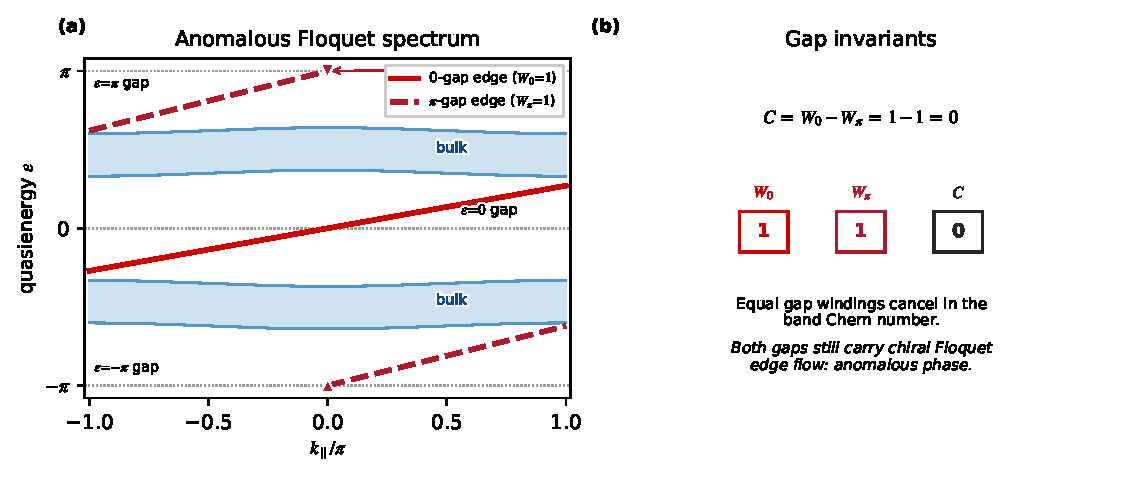
\includegraphics[width=0.92\textwidth]{figures/fig_ch13_floquet_quasienergy_step199.pdf}
  \caption{Anomalous Floquet topological insulator.
  \textbf{(a)}~Quasienergy spectrum in the reduced Floquet Brillouin
  zone $\varepsilon\in[-\pi,\pi]$ (we set $T=1$ so the zone boundaries
  lie at $\pm\pi$; in dimensional units the gap sits at
  $\varepsilon=\pi/T$).  Two bulk bands (blue shading) are
  separated by a wide gap at $\varepsilon=0$ and a narrower gap at
  $\varepsilon=\pm\pi$.  A chiral 0-gap edge mode (solid red) crosses
  the central gap with winding number $W_0=1$.  A chiral $\pi$-gap
  edge mode (dashed dark red) traverses the gap at $\varepsilon=\pm\pi$
  with $W_\pi=1$; the two dashed segments are the \emph{same} branch,
  connected by the periodicity $\varepsilon \equiv \varepsilon + 2\pi$
  (triangle markers indicate the identification point at $k_\parallel=0$).
  \textbf{(b)}~Gap invariants: the band Chern number
  $C = W_0 - W_\pi = 1 - 1 = 0$ vanishes even though both gaps carry
  chiral edge flow---this is the defining signature of the anomalous
  Floquet phase \cite{rudner2013anomalous}.}
  \label{fig:ch13-floquet-quasienergy}
\end{figure}


\section{Photonic Floquet realisations}
\label{sec:ch13-realisations}

\subsection{Helical waveguide arrays}
\label{sec:ch13-waveguide-arrays}

The first experimental demonstration of photonic Floquet topology was
achieved by Rechtsman et~al.\ (2013) using helical waveguide arrays
\cite{rechtsman2013photonica,maczewsky2017observation,yang2020photonic}.  In this elegant experiment, the
propagation axis $z$ plays the role of time, and the waveguide array
forms a 2D lattice in the transverse $(x,y)$ plane.  Each waveguide is
helically curved, so its transverse position oscillates periodically
along $z$.  The result is a $z$-periodic potential that creates a Floquet
system in the paraxial approximation.

The experiment demonstrated topological edge states at the boundary of
the waveguide array, propagating unidirectionally along the edge.  The
edge modes were robust to deliberate defects introduced by removing
individual waveguides.

\subsection{Deriving the paraxial equation from Maxwell's equations}
\label{sec:ch13-paraxial}

To maintain the Maxwell-first spirit of this book, we derive the
paraxial approximation from the Helmholtz equation rather than
postulating it by analogy with quantum mechanics.

Consider a monochromatic beam at frequency $\omega$ propagating
primarily along $z$ in a medium with refractive index
$n(\rvec_\perp,z)=n_0+\delta n(\rvec_\perp,z)$, where
$|\delta n|\ll n_0$.  The electric field can be written as
$E(\rvec)=\psi(\rvec_\perp,z)\ee^{\ii k_0 z}$, where
$k_0=n_0\omega/c$ is the carrier wavevector and $\psi$ is a slowly
varying envelope.

Substituting into the Helmholtz equation
$\nabla^2 E + k_0^2 n^2/n_0^2\,E = 0$ and neglecting the second
derivative $\partial^2\psi/\partial z^2$ (the paraxial approximation,
valid when $|\partial_z\psi|\ll k_0|\psi|$):
\begin{equation}\label{eq:ch13-paraxial}
  \boxed{%
  \ii\pderiv{\psi}{z}
  = -\frac{1}{2k_0}\nabla_\perp^2\psi
  - \frac{k_0\,\delta n(\rvec_\perp,z)}{n_0}\,\psi\,.}
\end{equation}
This has the same mathematical form as the time-dependent
Schr\"odinger equation, with the identifications: $z\leftrightarrow t$,
$1/(2k_0)\leftrightarrow\hbar/(2m)$, and
$-k_0\delta n/n_0\leftrightarrow V(\rvec)$.

When the waveguide pattern is periodic in $z$ with period $\Lambda$,
this is precisely a Floquet problem with
$\Omega_{\mathrm{mod}}=2\pi/\Lambda$ and time replaced by $z$.

\subsection{Quantitative parameters for the Rechtsman experiment}
\label{sec:ch13-rechtsman-params}

The Rechtsman waveguide array was fabricated by femtosecond-laser
direct writing in borosilicate glass ($n_0=1.46$) at wavelength
$\lambda=633\;\mathrm{nm}$ \cite{rechtsman2013photonica}.  The key
experimental parameters are: helical radius $R_h=8\;\mu\mathrm{m}$,
helix pitch $\Lambda=1\;\mathrm{cm}$, inter-waveguide spacing
$d=22\;\mu\mathrm{m}$, and refractive-index contrast
$\Delta n\approx 6\times 10^{-4}$.

The carrier wavenumber is
$k_0=2\pi n_0/\lambda\approx 1.45\times 10^7\;\mathrm{m}^{-1}$.
The coupling coefficient between nearest-neighbour waveguides is
$J\approx 0.6\;\mathrm{cm}^{-1}$, determined by the evanescent
overlap at spacing $d$.

The helix introduces an effective vector potential
$\mathbf{A}_{\mathrm{eff}}(z)
=k_0\,R_h\,\Omega_h\bigl(-\sin\Omega_h z,\,\cos\Omega_h z\bigr)$,
where $\Omega_h=2\pi/\Lambda$ is the helix angular frequency.  The
magnitude of the effective gauge field is
$|A_{\mathrm{eff}}|=k_0\,R_h\,\Omega_h
\approx 1.45\times 10^7\times 8\times 10^{-6}\times 628
\approx 73\;\mathrm{m}^{-1}$.
The effective flux per plaquette is
$\Phi=|A_{\mathrm{eff}}|\,d\approx 73\times 22\times 10^{-6}
\approx 1.6\times 10^{-3}\;\mathrm{rad}$---a small flux that
nonetheless produces a measurable topological gap because of the
large number of modulation periods over the sample length
($L/\Lambda=5$--$10$).

The topological gap in the Floquet quasi-energy spectrum is
$\Delta\varepsilon\approx 2\Phi\,J\approx 0.002\;\mathrm{cm}^{-1}$.
The edge-mode localisation length is
$\xi\approx 1/\Phi\times d\approx 17\;\mu\mathrm{m}$, comparable
to the inter-waveguide spacing, confirming strong edge localisation
\cite{ozawa2018topological,maczewsky2017observation}.

\subsection{The Magnus expansion and effective static Hamiltonian}
\label{sec:ch13-magnus}

For a periodically driven system $H(t)=H(t+T)$, the Floquet operator
$F=\mathcal{T}\exp(-\ii\int_0^T H(t)\,\dd t)$ defines the
stroboscopic evolution.  When the driving frequency
$\Omega_{\mathrm{mod}}$ is much larger than the bandwidth of the
static Hamiltonian, the Magnus expansion provides a systematic
perturbative construction of an effective static Hamiltonian
$H_{\mathrm{eff}}$ such that $F=\exp(-\ii H_{\mathrm{eff}}T)$.

The first two terms are
\begin{align}
  H_{\mathrm{eff}}^{(0)} &= \frac{1}{T}\int_0^T H(t)\,\dd t\,,
  \label{eq:ch13-magnus-0}\\
  H_{\mathrm{eff}}^{(1)} &= \frac{1}{2\ii T}\int_0^T\!\!\dd t_1
  \int_0^{t_1}\!\!\dd t_2\;[H(t_1),H(t_2)]\,.
  \label{eq:ch13-magnus-1}
\end{align}
The zeroth-order term is the time average, which is time-reversal
symmetric if $H(t)$ is.  The first-order correction involves the
commutator of $H$ at different times and generically breaks
time-reversal symmetry even if the instantaneous $H(t)$ preserves
it \cite{kitagawa2010topological,ozawa2018topological}.  This is the
mechanism by which periodic driving creates an effective gauge field.

For the helical-waveguide model, $H(t)$ is the hopping Hamiltonian
with periodically rotating coupling phases.  The zeroth-order term
gives the static nearest-neighbour hopping, and the first-order
commutator produces the desired Peierls phases with flux $\Phi$ per
plaquette.

\subsection{Convergence and heating}
\label{sec:ch13-convergence}

The Magnus expansion converges when the local norm
$\|H(t)\|\cdot T<\pi$, which requires the driving frequency to exceed
the bandwidth.  When this condition is marginally satisfied, the
effective Hamiltonian receives significant corrections at each order,
and the Floquet bands can differ qualitatively from the truncated
Magnus prediction.

In photonic systems, ``heating'' (the uncontrolled population of
high-energy Floquet replicas) is less problematic than in electronic
systems because photonic systems are classical and do not thermalise.
However, multiphoton resonances between Floquet replicas can produce
spurious gaps and flat bands that complicate the interpretation of
the quasi-energy spectrum \cite{price2022roadmap}.

\section{Connection to synthetic dimensions}
\label{sec:ch13-synthetic-connection}

The Floquet approach and the synthetic-dimension approach
(Chapter~\ref{ch:synthetic-dimensions}) are closely related.  Both use
temporal modulation to create effective gauge fields for photons.  The
key difference is the degree of freedom that plays the role of the
extra spatial dimension: in Floquet systems, the modulation creates a
$z$-periodic potential in real space; in synthetic-dimension systems,
the modulation couples discrete frequency modes into a lattice along
the frequency axis.

Mathematically, the connection becomes precise in the Floquet--Bloch
representation: the Fourier harmonic index $m$ in the Floquet expansion
\eqref{eq:ch13-fourier-expansion} plays the same role as the
synthetic-dimension site index in the ring-resonator frequency lattice
of Chapter~\ref{ch:synthetic-dimensions}.  The inter-harmonic coupling
$\Mmat_{m-m'}$ is the synthetic-dimension hopping, and the Floquet
quasi-energy $\varepsilon$ maps to the synthetic-dimension Bloch
momentum \cite{ozawa2018topological,price2022roadmap}.

\subsection{Coupled resonator networks}
\label{sec:ch13-resonators}

An alternative Floquet realisation uses networks of ring resonators with
time-modulated coupling, as proposed by Fang, Yu, and Fan (2012)
\cite{ozawa2018topological}.  The
modulation phases create effective magnetic fluxes through the
plaquettes, as described in \secref{sec:ch13-gauge-fields}.  This
approach allows direct electrical control of the effective gauge field
and has been demonstrated at microwave and radio frequencies.

\subsection{Acousto-optic implementations}
\label{sec:ch13-acousto-optic}

Acoustic waves propagating through an optical medium create a
travelling refractive-index grating that can serve as the temporal
modulation.  The acoustic frequency sets $\Omega_{\mathrm{mod}}$, and
the acoustic wavevector provides the spatial modulation pattern.  This
approach has been proposed for creating photonic Floquet topological
phases at optical frequencies.

\subsection{Anomalous Floquet topology: a concrete model}
\label{sec:ch13-afti-model}

To make the anomalous Floquet topological insulator concrete, consider
the periodically driven Haldane model studied by Kitagawa et~al.
\cite{kitagawa2010topological}.  The driving protocol consists of
five steps per period $T$, each activating one of the hopping
amplitudes of a honeycomb lattice in sequence.  In the high-frequency
limit $JT\ll 1$, the effective Floquet Hamiltonian reproduces the
static Haldane model with complex next-nearest-neighbour hopping.  But
in the resonant regime $JT\sim 1$, a richer phase diagram appears:
the Chern numbers of all Floquet bands can vanish simultaneously while
the winding numbers \eqref{eq:ch13-winding} at both $\varepsilon=0$
and $\varepsilon=\Omega_{\mathrm{mod}}/2$ are nonzero.  This is the
AFTI phase, confirmed experimentally by Maczewsky et~al.
\cite{maczewsky2017observation} in a laser-written waveguide array.

The experimental signature is striking: edge modes exist in
\emph{every} quasi-energy gap, even though no bulk band carries a
nonzero Chern number.  This was verified by exciting the edge of the
waveguide array with a focused beam and observing unidirectional
propagation along the boundary at both gap centres.

\section{Comparison with static topology}
\label{sec:ch13-comparison}

The static and Floquet approaches to photonic topology have
complementary strengths and limitations.

In static topological photonic crystals, the symmetry breaking is
permanent and built into the material (magneto-optical response).  The
topological protection is absolute within the gap, and the system
requires no external drive.  However, the gap width is limited by the
strength of the material response, and the topological properties
cannot be dynamically reconfigured.

In Floquet topological photonic systems, the symmetry breaking is
created by the temporal modulation and can be turned on, off, or
reconfigured by changing the modulation parameters.  The system can
access topological phases (such as the AFTI) that have no static
analog.  However, the modulation frequency sets an energy scale: for
wide topological gaps, fast modulation is needed, which becomes
technically challenging at optical frequencies.  Furthermore, Floquet
systems are inherently driven and may suffer from heating effects
(absorption of modulation energy) over long times.

\section{Anomalous Floquet topological insulator}
\label{sec:ch13-anomalous-floquet}

A remarkable feature of Floquet systems is the existence of topological
phases that have no static counterpart.  In a static 2D system, the
bulk-edge correspondence guarantees that the number of chiral edge
modes in a gap equals the sum of the Chern numbers of the bands below
the gap.  In a Floquet system, this correspondence can fail: a system
can have chiral edge modes in \emph{every} quasi-energy gap, even when
all the bands have zero Chern number.

\subsection{The winding number}
\label{sec:ch13-winding-number}

The anomalous Floquet phase is characterised by a winding number
$W_\varepsilon$ defined at each quasi-energy gap:
\begin{equation}\label{eq:ch13-winding-number}
  W_\varepsilon
  = \frac{1}{8\pi^2}\int_0^T\!\!\dd t\int_{\mathrm{BZ}}
  \Tr\bigl[
  U^{-1}\partial_t U\,[U^{-1}\partial_{k_x}U,\,U^{-1}\partial_{k_y}U]
  \bigr]\,\dd^2 k\,,
\end{equation}
where $U(\kvec,t)$ is the time-evolution operator from $t=0$ to $t$.
This is a three-dimensional topological invariant that integrates over
the full $(\kvec,t)$ space, in contrast to the Chern number which
integrates only over $\kvec$.  The winding number $W_\varepsilon$
reduces to the Chern number in the high-frequency limit but captures
additional topology when the driving is strong
\cite{kitagawa2010topological,ozawa2018topological}.

\subsection{Experimental realisation}
\label{sec:ch13-anomalous-expt}

The anomalous Floquet topological insulator was first realised
experimentally in a photonic waveguide array by Maczewsky et~al.\
(2017).  The waveguide coupling was modulated periodically along the
propagation direction $z$ using a four-step driving protocol that
breaks all spatial symmetries while preserving the periodicity.  The
resulting quasi-energy band structure has zero Chern number in every
band, yet chiral edge modes appear in every quasi-energy gap.

The experiment used femtosecond-laser-written waveguides in fused
silica, with a driving period $\Lambda=6\;\mathrm{cm}$, inter-waveguide
spacing $d=25\;\mu\mathrm{m}$, and operating wavelength
$\lambda=633\;\mathrm{nm}$.  The edge modes were observed as
bright, unidirectional channels localised at the boundary of the
waveguide array, with the propagation direction reversing at the
quasi-energy $\varepsilon=\pi/T$ gap
\cite{maczewsky2017observation,price2022roadmap}.

\section{Other Floquet photonic platforms}
\label{sec:ch13-other-platforms}

Beyond waveguide arrays, Floquet ideas have been applied to several
other photonic systems.

Coupled ring-resonator lattices can implement Floquet topological
phases by engineering the round-trip phase in each resonator to
produce a synthetic time step.  The discrete nature of the round-trip
evolution naturally produces a Floquet structure, and the phase can
be tuned to achieve nontrivial winding numbers
\cite{ozawa2018topological}.

Acoustic and mechanical analogs of Floquet photonic systems have been
demonstrated using time-modulated resonator lattices, where the
modulation frequency plays the role of the driving and the acoustic
pressure field plays the role of the electromagnetic field.  These
experiments confirm the universality of the Floquet topological
mechanism across wave physics \cite{price2022roadmap}.

The connection between Floquet driving and synthetic dimensions
(Chapter~\ref{ch:synthetic-dimensions}) provides yet another
perspective: the Floquet harmonics can be viewed as lattice sites
in a synthetic frequency dimension, and the anomalous Floquet phase
corresponds to a topological winding along the synthetic axis
\cite{ozawa2018topological}.

\section{Floquet engineering of gauge fields}
\label{sec:ch13-gauge-engineering}

Beyond creating topological band gaps, periodic driving can engineer
effective gauge fields that would be difficult or impossible to
realise in a static photonic structure.  The key principle is that
the time-averaged effect of a periodic modulation can produce an
effective Hamiltonian with complex hopping phases, even when the
instantaneous Hamiltonian is real.

\subsection{Effective magnetic flux from helical modulation}
\label{sec:ch13-helical-flux}

In the Rechtsman waveguide array (Section~\ref{sec:ch13-rechtsman-params}),
the helical trajectory of each waveguide produces an effective
vector potential $\mathbf{A}_{\mathrm{eff}}=k_0 R_h\Omega_z\hat{z}
\times\hat{r}$ in the co-moving frame, where $R_h$ is the helix
radius and $\Omega_z=2\pi/\Lambda$ is the spatial frequency.  The
effective magnetic flux per plaquette is
$\Phi_{\mathrm{eff}}=k_0 R_h\Omega_z\,a^2$, where $a$ is the lattice
constant.  For the experimental parameters ($R_h=8\;\mu\mathrm{m}$,
$\Lambda=1\;\mathrm{cm}$, $a=22\;\mu\mathrm{m}$,
$\lambda=633\;\mathrm{nm}$), this gives
$\Phi_{\mathrm{eff}}\approx 0.21\times 2\pi$
\cite{rechtsman2013photonica,ozawa2018topological}.

This effective flux is large enough to produce well-separated Chern
bands and observable edge states, but not so large that the Floquet
bands overlap (the high-frequency condition
$\hbar\Omega\gg J$ is satisfied).

\subsection{Four-step driving protocols}
\label{sec:ch13-four-step}

An alternative to continuous helical modulation is a discrete
step-wise protocol, in which the coupling between neighbouring
waveguides is turned on and off in a cyclic sequence.  Maczewsky
et~al.\ used a four-step protocol
($\mathrm{right}\to\mathrm{up}\to\mathrm{left}\to\mathrm{down}$)
with each step occupying one quarter of the driving period.  This
protocol breaks all spatial symmetries and produces an anomalous
Floquet topological insulator with zero Chern numbers but nonzero
winding numbers in every quasi-energy gap
\cite{maczewsky2017observation,kitagawa2010topological}.

\section{Heating and decoherence in Floquet photonic systems}
\label{sec:ch13-heating}

In electronic Floquet systems, periodic driving inevitably heats the
system toward infinite temperature, because the driving energy is
absorbed by the electrons.  This heating limits the lifetime of
Floquet topological phases and is a major obstacle for practical
applications.

In photonic Floquet systems, the situation is fundamentally different:
photons do not thermalise with each other (in the linear regime), so
there is no analog of Floquet heating.  The periodic modulation
simply produces a time-independent effective band structure, and the
``Floquet topological'' phase is stable indefinitely as long as the
modulation is maintained.

Decoherence in photonic Floquet systems arises from material
absorption and radiation loss, not from thermalisation.  These losses
give the Floquet edge modes a finite propagation length, analogous to
the loss-limited propagation in magneto-optical Chern insulators
(Chapter~\ref{ch:breaking-tr}).  For laser-written waveguides in fused
silica, the propagation loss is approximately
$0.5\;\mathrm{dB/cm}$, allowing edge-mode observation over
$\sim 10\;\mathrm{cm}$ propagation lengths
\cite{rechtsman2013photonica,price2022roadmap}.

\section{Floquet topological phases beyond the high-frequency limit}
\label{sec:ch13-beyond-high-freq}

Most of the analysis in this chapter has assumed the high-frequency
limit, where the driving frequency $\Omega$ is much larger than the
bandwidth $W$ of the instantaneous Hamiltonian: $\hbar\Omega\gg W$.
In this limit, the Floquet quasi-energy bands are well separated and
the effective Hamiltonian $H_{\mathrm{eff}}$ is accurately
approximated by the leading terms of the Magnus expansion
(Section~\ref{sec:ch13-magnus}).

\subsection{Resonant driving and Floquet band inversions}
\label{sec:ch13-resonant}

When $\hbar\Omega$ is comparable to $W$, resonances between Floquet
replicas produce band inversions that cannot be captured by the
effective Hamiltonian.  At these resonances, the quasi-energy bands
hybridise strongly, and the topology of the Floquet spectrum can
change discontinuously.

For the Rechtsman waveguide array, the high-frequency condition is
$\Omega\gg 2\pi v_D/a$, where $v_D$ is the Dirac velocity and $a$
is the lattice constant.  With the experimental parameters
($\Lambda=1\;\mathrm{cm}$, $a=22\;\mu\mathrm{m}$, $v_D\approx 10^5
\;\mathrm{m/s}$), this gives $\hbar\Omega/(2\pi v_D/a)\approx 20$,
well within the high-frequency regime.  However, for shorter driving
periods ($\Lambda\lesssim 1\;\mathrm{mm}$), resonant effects become
important and can produce additional topological transitions
\cite{rechtsman2013photonica,kitagawa2010topological}.

\subsection{Floquet--Bloch band structure}
\label{sec:ch13-floquet-bloch-structure}

The full Floquet--Bloch band structure is obtained by diagonalising
the one-period evolution operator $U(\kvec,T)$ at each Bloch
wavevector.  The quasi-energies $\varepsilon_n(\kvec)$ are defined
modulo $2\pi/T$, creating a periodic ``quasi-energy Brillouin zone''
in addition to the spatial Brillouin zone.  The topology of each
quasi-energy gap is characterised independently by the Chern number
(for gaps that are also present in the static limit) or by the winding
number \eqref{eq:ch13-winding} (for anomalous gaps that have no
static counterpart)
\cite{ozawa2018topological,maczewsky2017observation}.

\section{Connection to time crystals}
\label{sec:ch13-time-crystals}

Floquet topological phases share a deep connection with discrete time
crystals: both arise from systems with periodic time dependence and
both exhibit spontaneous breaking of the discrete time-translation
symmetry.  In a Floquet topological insulator, the edge modes
oscillate at frequencies that are subharmonics of the driving
frequency---a hallmark of discrete time-crystalline order.

In photonic systems, this connection has been explored in coupled
resonator networks where the edge modes spontaneously lock to a
subharmonic of the driving frequency, producing a ``topological time
crystal'' that is robust against perturbations.  The topological
protection ensures that the time-crystalline order is stable against
disorder that does not close the quasi-energy gap
\cite{price2022roadmap,ozawa2018topological}.

\section{Anomalous phases beyond band Chern numbers}
\label{sec:ch13-anomalous-beyond-chern}

One of the most striking predictions of Floquet topological theory
is the existence of \emph{anomalous} topological phases: driven
systems that support chiral edge states even when \emph{all}
quasi-energy-band Chern numbers vanish.  This phenomenon has no
static analogue and reveals the fundamentally richer topology of
periodically driven systems.

\subsection{Why static invariants fail}
\label{sec:ch13-anomalous-why}

In a static topological insulator, the number of chiral edge modes in
a gap equals the sum of Chern numbers of all bands below that gap.
In a Floquet system, the quasi-energy spectrum is periodic with period
$\Omega$, so there are two distinct gaps: one near quasi-energy $0$
and one near $\Omega/2$.  A band with Chern number $C$ contributes
edge modes to both gaps, and the net count in each gap depends on
how~$C$ is distributed between the two zone boundaries.

The anomalous phase arises when all quasi-energy bands have $C=0$, yet
chiral edge modes exist in one or both gaps.  This is possible because
the time-evolution operator $U(\kvec,T)$ encodes topological
information not captured by the instantaneous band Chern numbers
\cite{nathan2015topological,kitagawa2010topological}.

\subsection{The winding number invariant}
\label{sec:ch13-winding-invariant}

The correct topological invariant for Floquet systems was identified
by Rudner, Lindner, Berg, and Levin, who showed that the number of
chiral edge modes in the gap at quasi-energy~$\varepsilon$ is
determined by a \emph{winding number} $W_\varepsilon$ constructed from
the full time-dependent evolution operator $U(\kvec,t)$ for
$0\le t\le T$.

Define the unitary evolution operator from time zero to time $t$:
$U(\kvec,t)=\mathcal{T}\exp\bigl[-\ii\int_0^t
H(\kvec,t')\,\dd t'\bigr]$.  The winding number for the gap at
$\varepsilon$ is
\begin{equation}\label{eq:ch13-rudner-winding}
  W_\varepsilon
  = \frac{1}{8\pi^2}\int_0^T\!\dd t\int_{\mathrm{BZ}}\!\dd^2k\;
  \operatorname{Tr}\bigl[
  U^\dagger\partial_t U\,
  [U^\dagger\partial_{k_x}U,\,U^\dagger\partial_{k_y}U]
  \bigr]
  - \sum_{n:\,\varepsilon_n<\varepsilon} C_n\,.
\end{equation}
The first term is a three-dimensional winding number of the map
$U:\mathrm{BZ}\times[0,T]\to U(N)$; the subtracted sum removes the
conventional Chern-number contribution.  The winding number is an
integer and equals the number of anomalous chiral edge modes---those
that arise from the micromotion during the drive cycle rather than
from the stroboscopic band topology
\cite{nathan2015topological,ozawa2018topological}.

Physically, \eqref{eq:ch13-rudner-winding} captures the fact that edge
modes can be ``pumped'' across a gap during each drive cycle, even if
the Floquet bands carry zero net Chern number.  This pumping mechanism
is the dynamical counterpart of the Thouless charge pump of
\chref{ch:one-dimension} \cite{thouless1982quantized}.

\subsection{Experimental observation in photonic lattices}
\label{sec:ch13-anomalous-exp}

The anomalous Floquet topological phase was observed by Mukherjee
et~al.\ in a laser-written waveguide lattice
\cite{mukherjee2017experimental}.  The experiment used the same
femtosecond-laser-inscription technique as the Rechtsman experiment
(\secref{sec:ch13-rechtsman-params}), but with a two-step driving
protocol designed to produce zero Chern numbers for all quasi-energy
bands while maintaining a nonzero winding number.

In the first half of the propagation period, nearest-neighbour
couplings along one bond direction were enhanced; in the second half,
couplings along the complementary bonds were enhanced.  The
stroboscopic band structure was topologically trivial, but the full
time-evolution operator wound nontrivially.

Chiral edge modes were observed propagating along the lattice
boundary, with intensity localised within 2--3 sites of the edge.
The transport was robust against intentional disorder of up to 10\%
of the lattice constant in waveguide positions.  These observations
directly confirmed the anomalous Floquet phase
\cite{mukherjee2017experimental}.

\subsection{Implications for reconfigurable photonic devices}
\label{sec:ch13-anomalous-implications}

Because the topological protection in anomalous Floquet phases arises
from the driving protocol rather than from the static band structure,
it can be switched on and off by changing the modulation pattern.
This enables dynamically reconfigurable topological waveguides,
routers, and filters that can be reprogrammed without modifying the
physical structure.

Furthermore, a Floquet system with $N$ quasi-energy bands has $N$
independent winding numbers (one per gap), compared to $N-1$
independent Chern numbers.  This additional topological degree of
freedom can be exploited to engineer multi-channel edge transport with
independently controllable numbers of edge modes in different
quasi-energy windows \cite{ozawa2018topological}.

\begin{figure}[t]
  \centering
  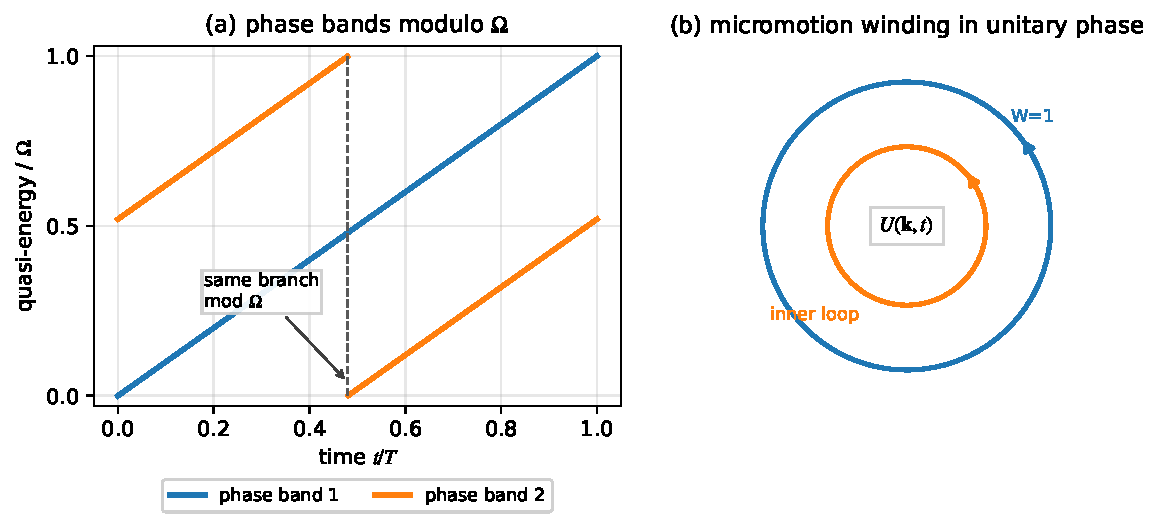
\includegraphics[width=0.88\textwidth]{figures/fig_ch13_floquet_winding.pdf}
  \caption{Floquet topology depends on micromotion during the whole period,
  not only on the stroboscopic band Chern numbers.  Phase bands can wind
  around the quasi-energy zone during one drive cycle, and the resulting
  map $U(\mathbf{k},t)$ over $\mathrm{BZ}\times S^1$ is measured by the
  gap winding invariant $W_\varepsilon$.}
  \label{fig:ch13-floquet-winding}
\end{figure}

\section*{Exercises}

\begin{exercise}
  Derive the paraxial equation \eqref{eq:ch13-paraxial} from the
  Helmholtz equation by writing $E=\psi\ee^{\ii k_0 z}$ and
  neglecting $\partial^2\psi/\partial z^2$.  State the conditions
  under which the approximation is valid and estimate the error for
  a beam with divergence angle $\theta$.
\end{exercise}

\begin{exercise}
  For a 1D lattice of coupled resonators with nearest-neighbour hopping
  $J_{ij}=J_0\ee^{\ii\phi_{ij}}$, compute the effective magnetic flux
  per plaquette for a square lattice with uniform phase
  $\phi_{ij}=\alpha$ along $x$ and $\phi_{ij}=0$ along $y$.  For what
  values of $\alpha$ is time-reversal symmetry effectively broken?
\end{exercise}

\begin{exercise}
  Show that the Floquet operator $F(\kvec)=U(\kvec,T)$ is unitary, and
  that its eigenvalues $\ee^{-\ii\varepsilon_n T}$ lie on the unit
  circle.  Interpret the quasi-energy $\varepsilon_n$ as the argument
  of these eigenvalues.
\end{exercise}

\begin{exercise}
  Explain why an anomalous Floquet topological insulator (all band
  Chern numbers zero, but edge modes present) is impossible in a static
  system.  What additional topological invariant distinguishes the
  AFTI from a trivial insulator?
\end{exercise}

\begin{exercise}
  In the Rechtsman waveguide experiment, the waveguides are helically
  curved with helix radius $R=8\;\mu\mathrm{m}$ and pitch
  $\Lambda=1\;\mathrm{cm}$ in fused silica ($n_0=1.46$) at
  $\lambda=633\;\mathrm{nm}$.  Compute the effective modulation strength
  $\delta n_{\mathrm{eff}}\sim n_0 k_0 R^2(2\pi/\Lambda)^2$ and
  estimate the topological gap width relative to the coupling
  strength $J\sim 1\;\mathrm{cm}^{-1}$.
\end{exercise}

\begin{exercise}
  For a Floquet system with two bands and modulation period $T$,
  compute the winding number \eqref{eq:ch13-winding} for a specific
  model: $H(k,t) = [J_1+J_2\cos(k)]\sigma_x + J_2\sin(k)\sigma_y
  + \Delta(t)\sigma_z$ with $\Delta(t)=\Delta_0\cos(\Omega t)$.  Under
  what conditions is the winding number nonzero?
\end{exercise}
